\chapter{Boundary conditon analysis in non level set simulations}

\comment{this appendix is temporary, it may be deleted later}

We want to understand the consequence of removing the no-slip boundary condition at the \emph{M-A} boundary and compare the effect on macrosegregation. 
For computations without level set, as previously done in chapter 4 for the \emph{Tsolver}'s validation in convection-diffusion regimes, 
a no-slip condition was applied for all domain boundaries.
However, this is not readily implemented with the level set method which considers the local interface velocity for its transport.
In \cref{fig:slipbc_2800,fig:slipbc_7000}, we compare at 2800 s and 7000 s the differences between a no-slip condition on the top boundary 
and a free-slip tangential condition, assuming zero normal velocity. 

%-----------------
\begin{figure}[htbp]
\centering
   %------------
  \begin{subfigure}[t]{0.4\textwidth}
    \centering
  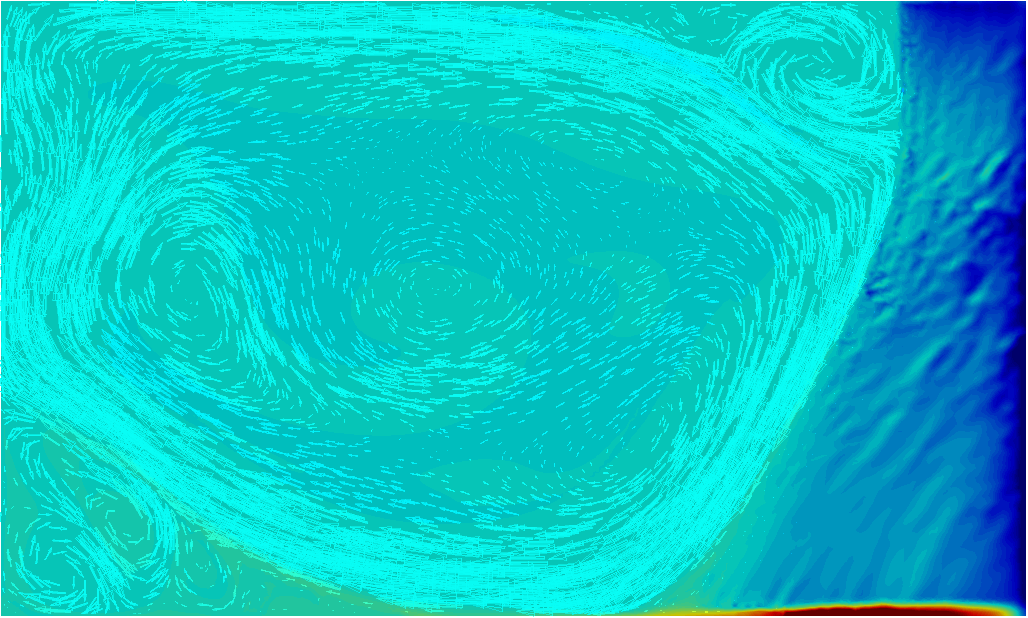
\includegraphics[width=\textwidth]{Chapter5/Graphics/2d/ref_2800s_nosliptop.png}
  \caption{}
    \label{fig:noslip2800}
  \end{subfigure}
  %------------------------------
  \begin{subfigure}[t]{0.15\textwidth}
    \centering
  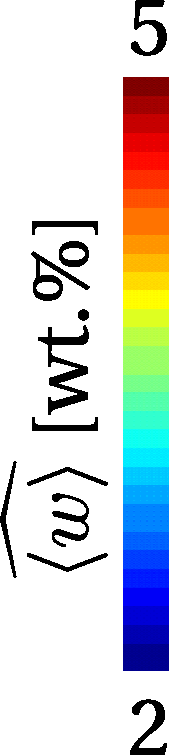
\includegraphics[width=0.3\textwidth]{Chapter5/Graphics/2d/colorbar_w.pdf}
  \end{subfigure}
  %------------------------------
  \begin{subfigure}[t]{0.4\textwidth}
    \centering
  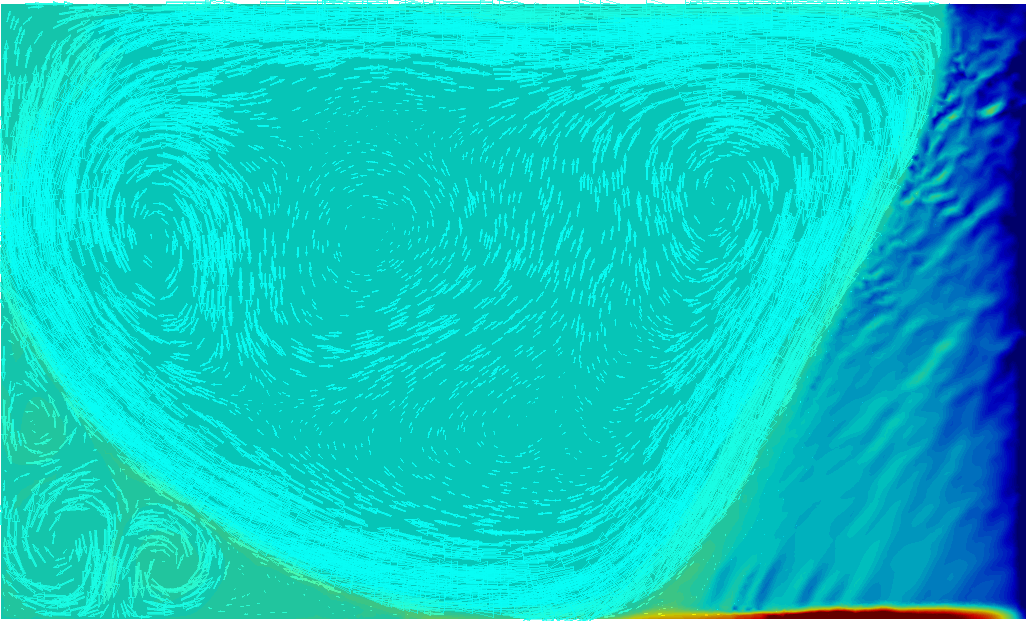
\includegraphics[width=\textwidth]{Chapter5/Graphics/2d/ref_2800s_sliptop.png}
  \caption{}
    \label{fig:freeslip2800}
  \end{subfigure}
   %------------
\caption{Comparison of two solidification with macrosegregation cases assuming (a) a no-slip condition on the upper boundary 
or (b) a tangential free-slip condition. The snapshots are taken at 2800 s.}
\label{fig:slipbc_2800}
\end{figure}
%------------------

%-----------------
\begin{figure}[htbp]
\centering
   %------------
  \begin{subfigure}[t]{0.4\textwidth}
    \centering
  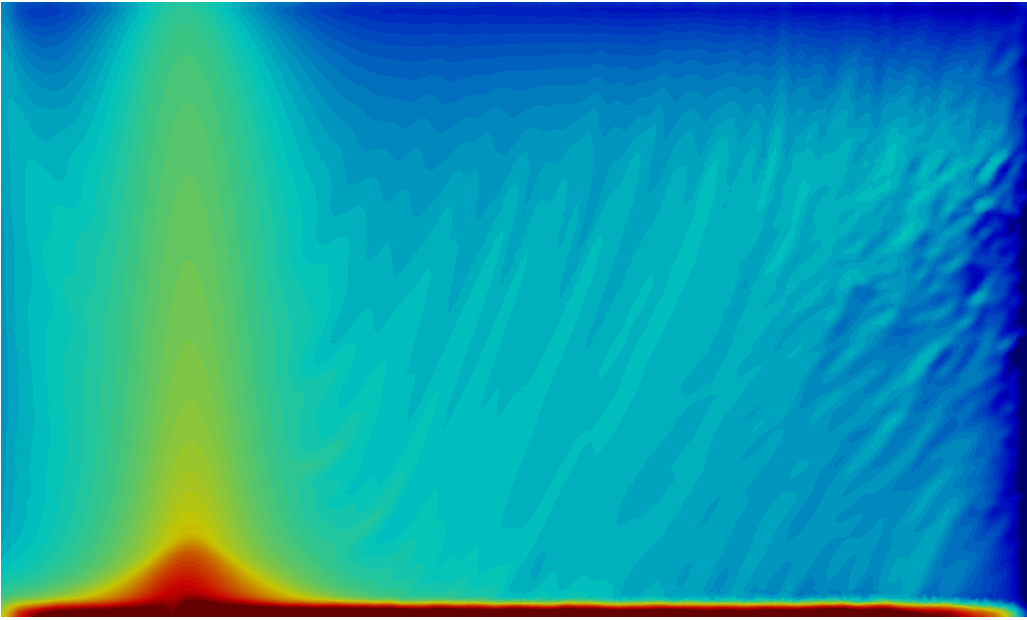
\includegraphics[width=\textwidth]{Chapter5/Graphics/2d/ref_7000s_nosliptop.png}
  \caption{}
    \label{fig:noslip7000}
  \end{subfigure}
  %------------------------------
  \begin{subfigure}[t]{0.15\textwidth}
    \centering
  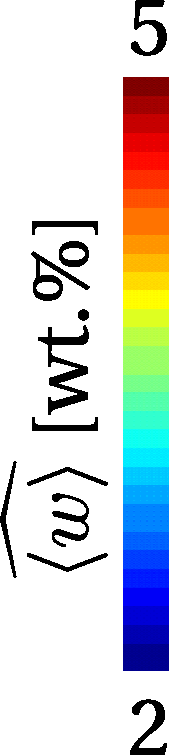
\includegraphics[width=0.3\textwidth]{Chapter5/Graphics/2d/colorbar_w.pdf}
  \end{subfigure}
  %------------------------------
  \begin{subfigure}[t]{0.4\textwidth}
    \centering
  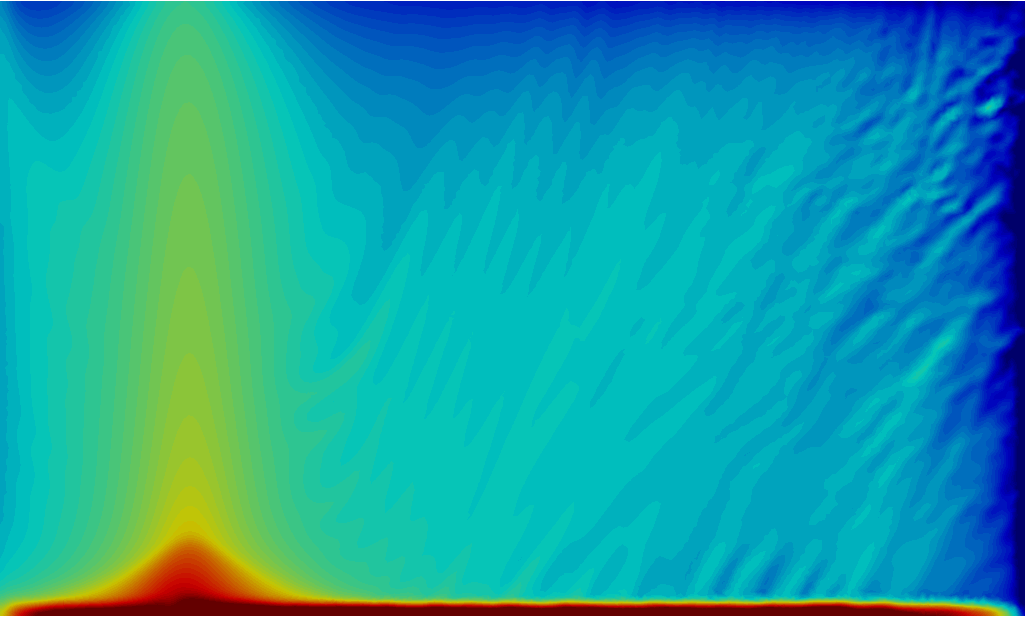
\includegraphics[width=\textwidth]{Chapter5/Graphics/2d/ref_7000s_sliptop.png}
  \caption{}
    \label{fig:freeslip7000}
  \end{subfigure}
   %------------
\caption{Comparison of two solidification with macrosegregation cases assuming (a) a no-slip condition on the upper boundary 
or (b) a tangential free-slip condition. The snapshots are taken at 7000 s.}
\label{fig:slipbc_7000}
\end{figure}
%------------------

In \cref{fig:slipbc_2800}, solidification is still at an early stage, at 2800 s. The main difference between \cref{fig:noslip2800} and 
\cref{fig:freeslip2800} is the flow pattern near the top interface. The no-slip wall acts a brake for the vicinity flow, 
deviating it downwards and allow a quicker solidification rate for the right upper part of the metal. The flow near the slip wall
in \cref{fig:freeslip2800} is not damped and therefore delays solidification of the upper corner where it impinges.
The different flow pattern creates a more pronounced negative segregation in the upper right corner of \cref{fig:noslip2800}, compared
to the same location in  \cref{fig:freeslip2800}. Later when solidification is complete at 7000 s (\cref{fig:slipbc_7000}), the overall
macrosegregation is more visible: expect for the previously mentioned difference in the corner segregation, no big differences are observed.
This means that when using the level set method, allowing the velocity to have non-zero values near the interface should not drastically  change the
predicted flow pattern and the subsequent macrosegregation.
% \section{Useful Expressions}
% \comment{ address a problem: attend to, apply oneself to, tackle, see to, deal with, confront, come to grips with, get down to, turn one's hand to, take in hand, undertake, concentrate on, focus on, devote oneself to
% "the selectmen failed to address the issue of subsidies" }
% \begin{itemize}
% \item  the basic premise = the basic argument is that ...
% \item A complication inherent in this approach is that
% \item an important objective of the present study is to
% \end{itemize}
